\documentclass[aspectratio=169, 10pt]{beamer}

\usetheme{focus}

% Paleta SupaClock, mantenida desde Entrega 3
\definecolor{main}{RGB}{57, 110, 184}
\definecolor{background}{RGB}{255, 255, 255}
\definecolor{accent}{RGB}{63, 185, 80}
\definecolor{warn}{RGB}{218, 54, 51}
\definecolor{softgray}{RGB}{245, 247, 250}
\definecolor{darkink}{RGB}{23, 32, 51}
\definecolor{muted}{RGB}{91, 102, 122}

\setbeamercolor{alerted text}{fg=warn}

\usepackage[spanish]{babel}
\usepackage[utf8]{inputenc}
\usepackage[T1]{fontenc}
\usepackage{graphicx}
\usepackage{booktabs}
\usepackage{array}
\usepackage{tikz}
\usepackage{pgfplots}
\pgfplotsset{compat=1.18}
\usetikzlibrary{shapes.geometric, arrows.meta, positioning, fit, backgrounds, calc, babel}

\setbeamerfont{itemize/enumerate body}{size=\small}
\setbeamerfont{itemize/enumerate subbody}{size=\footnotesize}
\setbeamerfont{block body}{size=\footnotesize}
\setbeamerfont{block title}{size=\small}

% Recursos: carpeta actual + bases visuales y técnicas de entregas anteriores.
\graphicspath{{./}{../Entrega2/}{../Entrega2/presentacion_v2/}{../Entrega3/}{../../mechanical/}{../../tools/}{../../hardware/SupaClock_Carrier/}{../../hardware/SupaClock_Carrier_v3/}}

\newcommand{\ok}{\textcolor{accent}{\textbf{OK}}}
\newcommand{\warnstate}{\textcolor{orange}{\textbf{En cierre}}}
\newcommand{\pending}{\textcolor{warn}{\textbf{Pendiente}}}
\newcommand{\metric}[2]{\textcolor{main}{\Large\textbf{#1}}\\[-0.02cm]{\scriptsize #2}}

\title{Wearable ``SupaClock''}
\subtitle{Entrega 4 \textbar{} Avance 90\%}
\date{\today}
\author{Grupo 10}
\institute{Ingenier\'ia El\'ectrica}
\titlegraphic{\hfill
\includegraphics[height=1.8cm]{logo.pdf}}

\begin{document}

\maketitle

\begin{frame}{Continuidad del proyecto}
    \begin{columns}[T]
        \column{0.47\textwidth}
        \footnotesize
        \textbf{Evoluci\'on por entregas}
        \begin{itemize}\itemsep0.10cm
            \item \textbf{Entrega 0--1}: problema, requisitos, arquitectura de alto nivel y alcance biom\'etrico.
            \item \textbf{Entrega 2}: sensores, firmware FreeRTOS, GUI, BLE y validaci\'on de subsistemas.
            \item \textbf{Entrega 3}: migraci\'on a XIAO ESP32-S3, carrier PCB, carcasa y ruta TinyML.
            \item \textbf{Entrega 4}: demostraci\'on del ECG en PCB, avances ML y cierre hacia el 100\%.
        \end{itemize}
        \column{0.53\textwidth}
        \begin{block}{Tesis de esta entrega}
            Ya no estamos validando componentes aislados: estamos mostrando un prototipo funcional al 90\%, con los riesgos principales concentrados en manufactura, carcasa final y validaci\'on repetible.
        \end{block}
        \vspace{0.2cm}
        \centering
        
\includegraphics[height=2.35cm]{supaclock_logo_e4.jpg}
    \end{columns}
\end{frame}

\begin{frame}{Objetivo de la Entrega 4}
    \begin{columns}[T]
        \column{0.58\textwidth}
        \footnotesize
        Esta presentaci\'on consolida el avance al 90\% y ordena el tramo final del proyecto.
        \vspace{0.25cm}
        \begin{itemize}\itemsep0.14cm
            \item Mostrar \textbf{ECG funcionando en la PCB}, con captura real y transmisi\'on hacia la app.
            \item Presentar los avances de \textbf{Machine Learning} para reconocimiento de actividad humana.
            \item Explicar la \textbf{PCB final fabricada en China}, orientada a reducir altura y mejorar repetibilidad.
            \item Definir qu\'e falta para cerrar el \textbf{100\%}: carcasa, validaci\'on, dataset y demo final.
        \end{itemize}
        \column{0.42\textwidth}
        \centering
        \begin{tikzpicture}
            \node[draw=accent, fill=accent!12, rounded corners=8pt, minimum width=4.0cm, minimum height=2.6cm] (box) {};
            \node[font=\Huge\bfseries, text=accent] at (box.center) {90\%};
            \node[font=\scriptsize, align=center, text=darkink] at ($(box.center)+(0,-1.05)$) {Prototipo funcional\\con cierre industrial pendiente};
        \end{tikzpicture}
        \vspace{0.25cm}
        \begin{alertblock}{Criterio de avance}
            \scriptsize El 10\% restante no es ``hacer que prenda'': es hacer que sea repetible, usable y validable como reloj cerrado.
        \end{alertblock}
    \end{columns}
\end{frame}

\begin{frame}{Estado del proyecto al 90\%}
    \scriptsize
    \centering
    \begin{tabular}{p{2.6cm}p{4.4cm}p{4.4cm}p{1.5cm}}
        \toprule
        \textbf{Bloque} & \textbf{Estado actual} & \textbf{Cierre hacia 100\%} & \textbf{Avance} \\
        \midrule
        ECG + PCB & Captura real desde AD8232 en carrier; streaming BLE a $\sim$500\,Hz. & Validar con carcasa cerrada, electrodos definitivos y ruido real. & \ok \\
        App + BLE & Dashboard, modo dev, REC IMU/ECG, consola y comandos. & Pulir experiencia de usuario y persistencia final de sesiones. & \ok \\
        Machine Learning & Validaci\'on inercial (clean/noisy) y an\'alisis de robustez. & Dataset final, data augmentation y cierre de inferencia Core 1. & \warnstate \\
        PCB final & Carrier validado; versiones v3/v4 orientadas a reglas JLCPCB. & DRC final, pedido, ensamble y bring-up de placa fabricada en China. & \warnstate \\
        Carcasa & Prototipo impreso permiti\'o detectar tolerancias, altura y contacto sensor-piel. & Redise\~no compacto alineado a PCB final y sensores. & \warnstate \\
        \bottomrule
    \end{tabular}
    \vspace{0.35cm}
    \begin{block}{Lectura del avance}
        \scriptsize El proyecto se mueve desde una demostraci\'on funcional de laboratorio hacia una unidad wearable repetible.
    \end{block}
\end{frame}

\section{ECG en PCB}

\begin{frame}{ECG funcionando en la PCB}
    \begin{columns}[T]
        \column{0.52\textwidth}
        \centering
        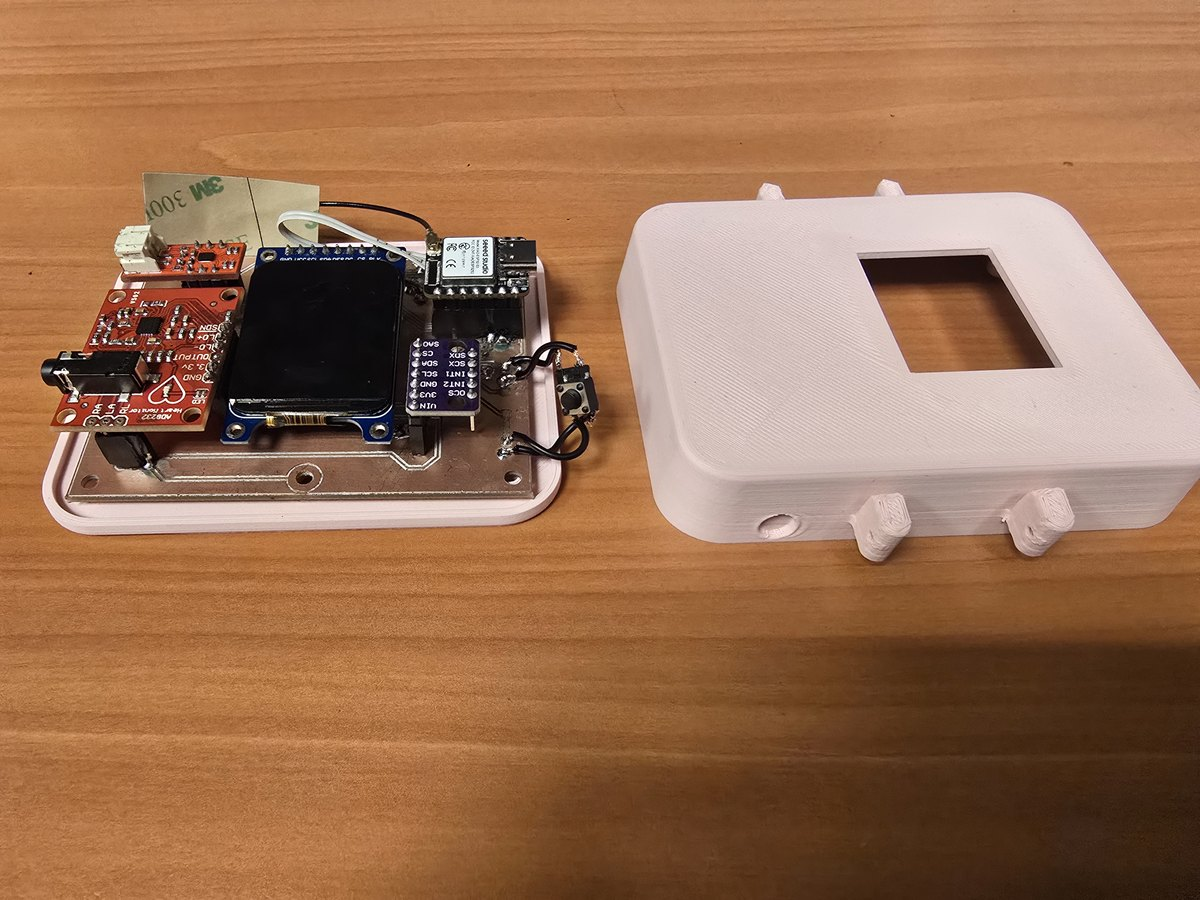
\includegraphics[width=\linewidth]{prototipopcb_e4.jpg}
        \vspace{0.08cm}
        \scriptsize Prototipo con PCB, XIAO ESP32-S3, AD8232, pantalla y carcasa impresa.
        \column{0.48\textwidth}
        \footnotesize
        \textbf{Qu\'e se valida}
        \begin{itemize}\itemsep0.12cm
            \item Ruta el\'ectrica: electrodos $\rightarrow$ AD8232 $\rightarrow$ ADC/DMA del ESP32-S3.
            \item Firmware capaz de activar/detener streaming ECG.
            \item App Flutter recibiendo paquetes BLE \texttt{0xFF03}.
            \item Registro local de se\~nal cruda para an\'alisis posterior.
        \end{itemize}
        \vspace{0.2cm}
        \begin{block}{Resultado central}
            \scriptsize El ECG ya no depende de protoboard: funciona desde la integraci\'on f\'isica del reloj.
        \end{block}
    \end{columns}
\end{frame}

\begin{frame}{Se\~nal ECG real: adquisici\'on y transmisi\'on}
    \begin{columns}[T]
        \column{0.68\textwidth}
        \centering
        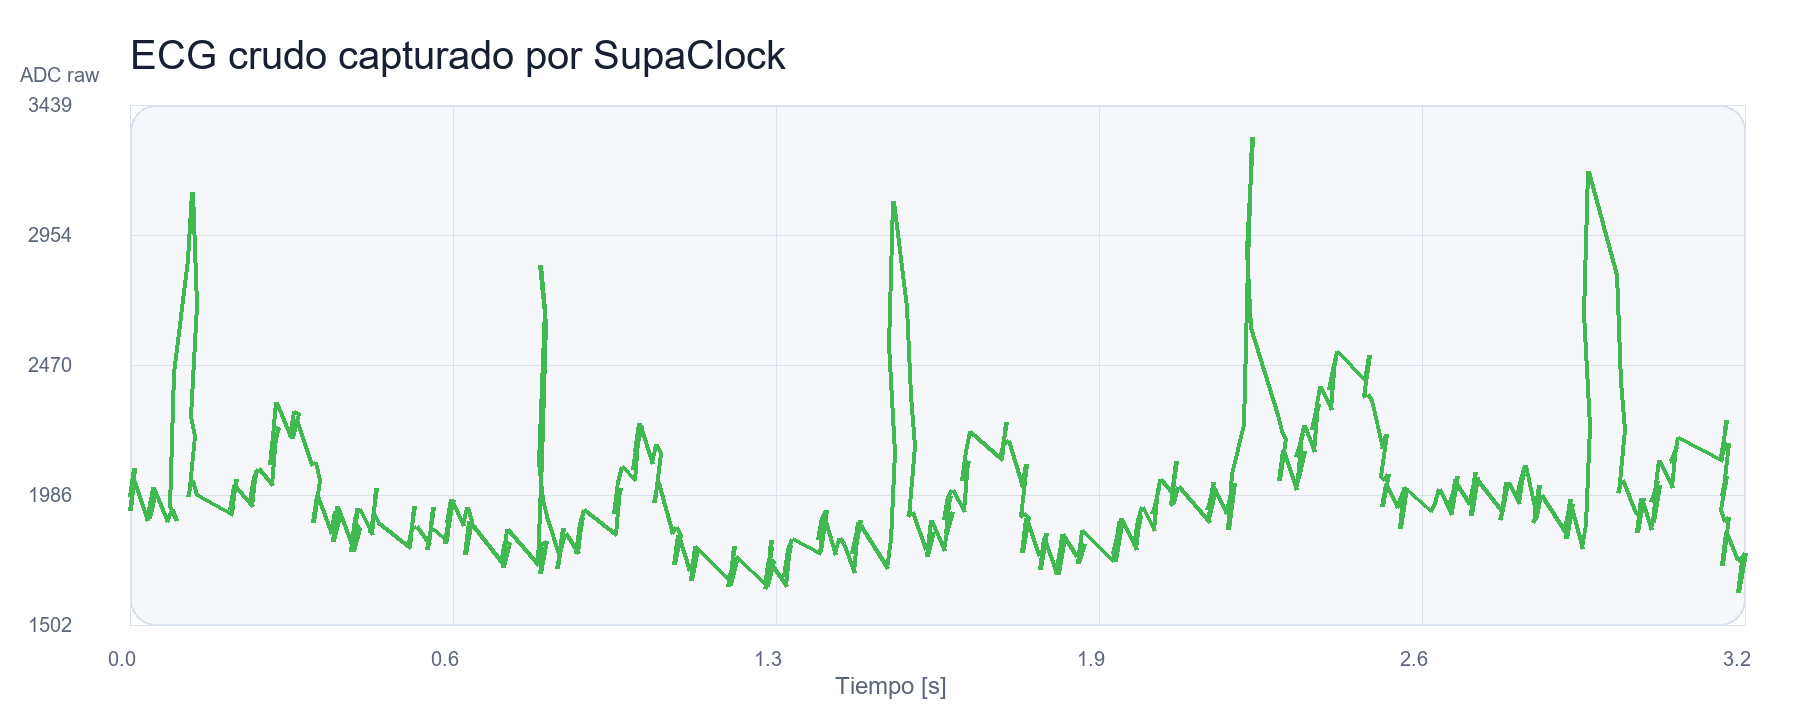
\includegraphics[width=\linewidth]{ecg_signal_20260618.png}
        \column{0.32\textwidth}
        \scriptsize
        \vspace{0.2cm}
        \metric{23.400}{muestras registradas}\\[0.35cm]
        \metric{46,8\,s}{duraci\'on capturada}\\[0.35cm]
        \metric{500,2\,Hz}{frecuencia estimada}\\[0.35cm]
        \metric{1143--3447}{rango ADC raw}\\[0.25cm]
        \begin{block}{Cadena validada}
            \scriptsize PCB/AD8232 $\rightarrow$ ADC/DMA $\rightarrow$ BLE 20 B (10$\times$int16) $\rightarrow$ Flutter $\rightarrow$ CSV/app.
        \end{block}
    \end{columns}
\end{frame}

\begin{frame}{BLE y app como banco de pruebas}
    \begin{columns}[T]
        \column{0.25\textwidth}
        \centering
        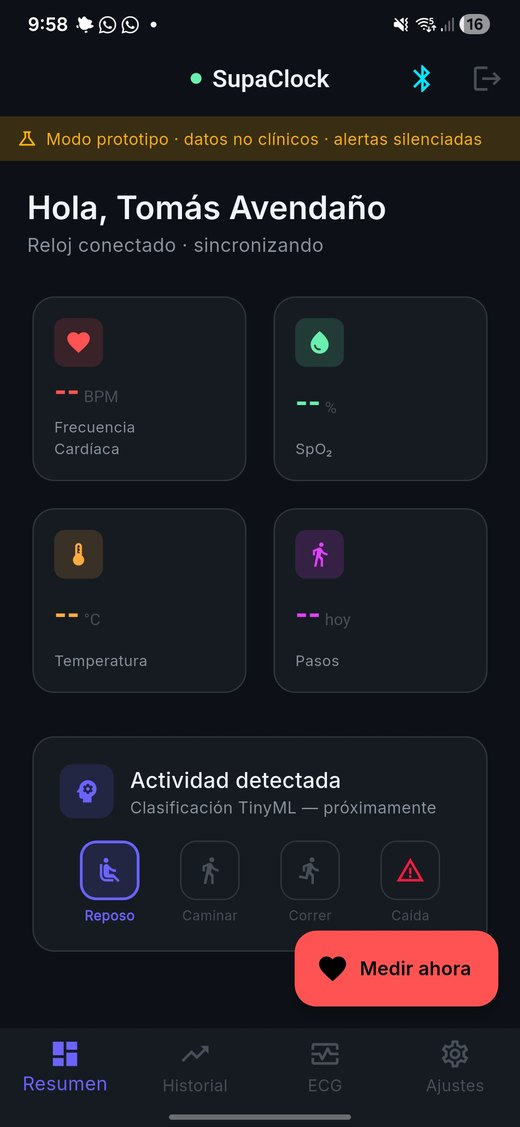
\includegraphics[height=5.0cm]{app_home_e4.jpg}
        \scriptsize Dashboard
        \column{0.25\textwidth}
        \centering
        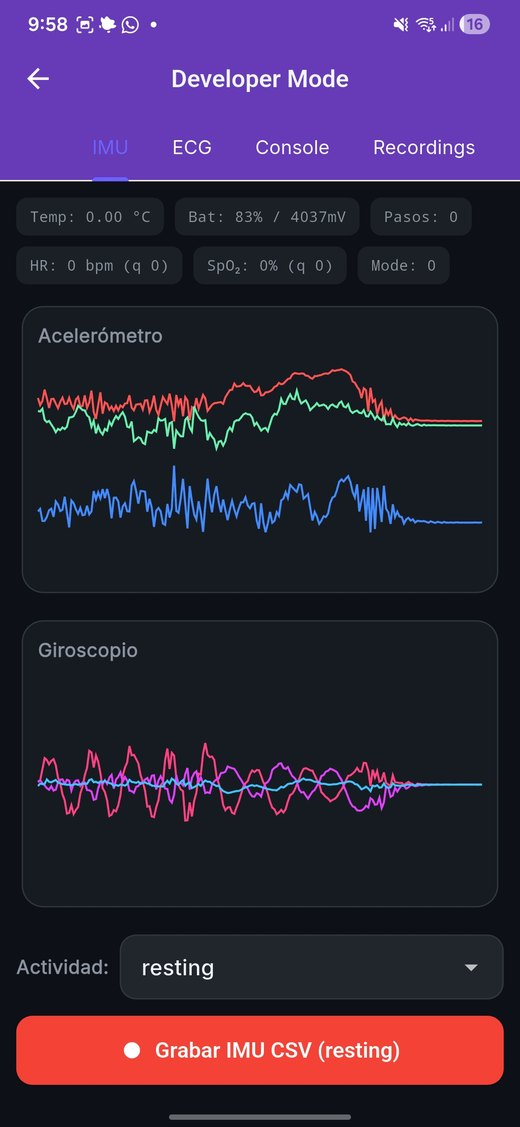
\includegraphics[height=5.0cm]{app_imu_e4.jpg}
        \scriptsize IMU en vivo
        \column{0.25\textwidth}
        \centering
        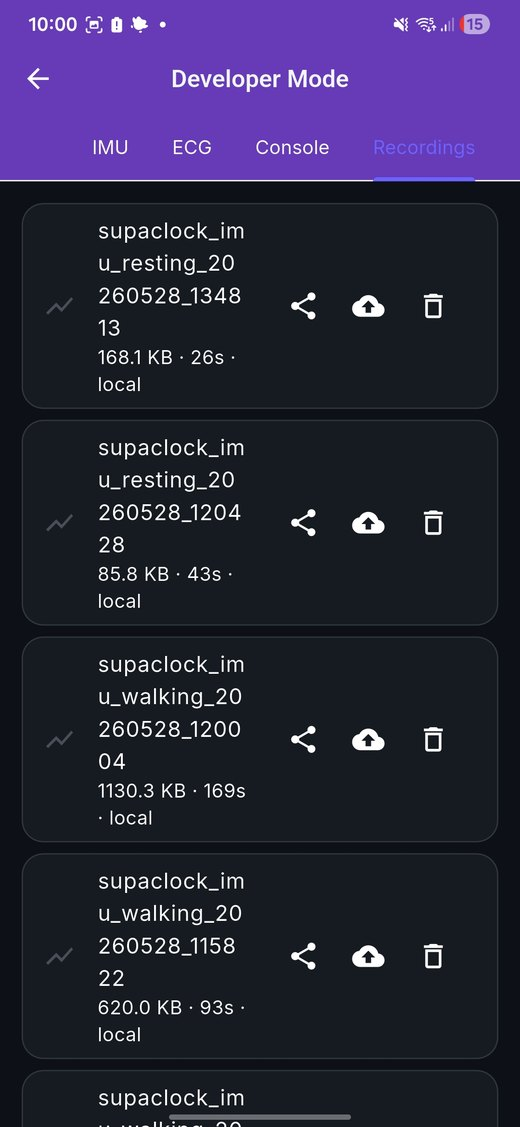
\includegraphics[height=5.0cm]{app_rec_e4.jpg}
        \scriptsize CSV etiquetado
        \column{0.25\textwidth}
        \scriptsize
        \textbf{Canales BLE}
        \vspace{0.08cm}
        \begin{tabular}{l l}
            \toprule
            \textbf{UUID} & \textbf{Uso} \\
            \midrule
            \texttt{FF01} & IMU raw \\
            \texttt{FF02} & TLV agregado \\
            \texttt{FF03} & ECG raw \\
            \texttt{FF04} & Comandos \\
            \bottomrule
        \end{tabular}
        \vspace{0.15cm}
        \begin{block}{Valor para el proyecto}
            \tiny La app permite probar, registrar y etiquetar datos sin depender de herramientas externas de consola.
        \end{block}
    \end{columns}
\end{frame}

\section{Machine Learning}

\begin{frame}{Evolución del Clasificador HAR (Upgrade del Modelo)}
    \begin{columns}[T]
        \column{0.50\textwidth}
        \footnotesize
        \textbf{El problema anterior (Umbrales)}
        \begin{itemize}\itemsep0.10cm
            \item Alta propensión a falsos positivos en reposo ante movimientos cotidianos (escribir, rascarse).
            \item Dificultad para discernir entre caminar y correr.
        \end{itemize}
        \vspace{0.2cm}
        \textbf{La solución (CNN 1D)}
        \begin{itemize}\itemsep0.10cm
            \item Extrae correlación espacio-temporal en 3 ejes.
            \item Ventana de 4\,s (200 muestras) filtra transitorios.
        \end{itemize}
        \column{0.50\textwidth}
        \footnotesize
        \textbf{Integración en SupaClock}
        \begin{itemize}\itemsep0.10cm
            \item **Inferencia en Core 1**: Ejecución asíncrona (FreeRTOS) que no interrumpe la GUI ni el BLE.
            \item **Ultra Latencia**: Inferencia $<10$\,ms optimizada por instrucciones vectoriales **ESP-NN**.
            \item **Estabilidad**: 99.52\% de precisión en estado de Reposo.
        \end{itemize}
    \end{columns}
\end{frame}

\begin{frame}{Arquitectura de la Red CNN 1D Embebida}
    \begin{columns}[T]
        \column{0.52\textwidth}
        \scriptsize
        \begin{itemize}\itemsep0.08cm
            \item \textbf{Entrada}: Tensor $200 \times 6$ (Acel/Giro a 50\,Hz) normalizado en rango $[-1.0, 1.0]$.
            \item \textbf{Cuerpo Convolucional (Extracción)}:
                \begin{itemize}\itemsep0.02cm
                    \item Conv1D (32 fil, k=5) + MaxPool: Rasgos inerciales.
                    \item Conv1D (64 fil, k=5) + MaxPool: Ciclos de marcha.
                    \item Conv1D (64 fil, k=3) + MaxPool: Rasgos rápidos.
                    \item Conv1D (128 fil, k=3): Patrones abstractos.
                \end{itemize}
            \item \textbf{Global Average Pooling (GAP)}: Promedia la dimensión temporal ($25 \times 128 \rightarrow 128$). Reduce parámetros densos de 3200 a 128, logrando un modelo de sólo 73\,KB.
            \item \textbf{Clasificador Final}: Capa Dense (64, relu) con Dropout (0.3) y salida Softmax de 4 clases (reposo, caminar, correr, caída).
        \end{itemize}
        
        \column{0.48\textwidth}
        \centering
        \begin{tikzpicture}[
            node distance=0.18cm,
            layer/.style={draw=main, fill=main!9, rounded corners=2pt, align=center, font=\tiny, minimum width=2.6cm, minimum height=0.32cm},
            pool/.style={layer, fill=accent!12, draw=accent},
            gap/.style={layer, fill=orange!15, draw=orange},
            dense/.style={layer, fill=purple!12, draw=purple},
            arr/.style={-Stealth, thick, main}
        ]
            \node[layer] (in) {Entrada: $200 \times 6$};
            \node[layer, below=of in] (c1) {Conv1D (32 fil, k=5) + MP};
            \node[layer, below=of c1] (c2) {Conv1D (64 fil, k=5) + MP};
            \node[layer, below=of c2] (c3) {Conv1D (64 fil, k=3) + MP};
            \node[layer, below=of c3] (c4) {Conv1D (128 fil, k=3)};
            \node[gap, below=of c4] (gap) {Global Average Pool (GAP)};
            \node[dense, below=of gap] (d1) {Dense (64) + Dropout (0.3)};
            \node[dense, below=of d1, fill=main!20, draw=main] (out) {Softmax (4 clases)};

            \draw[arr] (in) -- (c1);
            \draw[arr] (c1) -- (c2);
            \draw[arr] (c2) -- (c3);
            \draw[arr] (c3) -- (c4);
            \draw[arr] (c4) -- (gap);
            \draw[arr] (gap) -- (d1);
            \draw[arr] (d1) -- (out);
        \end{tikzpicture}
    \end{columns}
\end{frame}

\begin{frame}{Resultados de Inferencia: Comparación Clean vs Noisy}
    \scriptsize
    \centering
    \begin{tabular}{l c c c}
        \toprule
        \textbf{Modelo} & \textbf{TFLite (KB)} & \textbf{Acc. Clean (\%)} & \textbf{Acc. Noisy ($\sigma$=0.05) (\%)} \\
        \midrule
        \textbf{Model A} (Baseline) & 58.11 & 98.95\% & \textbf{98.16\%} (Excelente) \\
        \textbf{Model B} (Ancho + L2) & 188.32 & 98.29\% & \textbf{98.43\%} (Muy robusto) \\
        \textbf{Model C} (Profundo) & 73.09 & \textbf{98.82\%} & 94.88\% (Sensible) \\
        \bottomrule
    \end{tabular}
    \vspace{0.25cm}
    \begin{columns}[T]
        \column{0.50\textwidth}
        \scriptsize
        \textbf{Métricas por Clase (Model C - Clean)}:
        \begin{itemize}\itemsep0.05cm
            \item **Reposo**: Prec. 99.52\% / Recall 98.81\%
            \item **Caminar**: Prec. 99.10\% / Recall 99.55\%
            \item **Correr**: Prec. 95.87\% / Recall 97.48\%
        \end{itemize}
        \column{0.50\textwidth}
        \scriptsize
        \textbf{Validación Rigurosa}
        \begin{itemize}\itemsep0.05cm
            \item Evaluación en test set separado (20\%).
            \item Copia con ruido Gaussiano simula jitter real.
            \item Model C es eficiente pero sensible al ruido físico.
        \end{itemize}
    \end{columns}
\end{frame}

\begin{frame}{Análisis de Diseño: ¿Profundidad o Ancho?}
    \begin{columns}[T]
        \column{0.50\textwidth}
        \footnotesize
        \textbf{Más Filtros (Model B - Ancho)}
        \begin{itemize}\itemsep0.10cm
            \item Tamaño crece a 188.32\,KB (3.2x).
            \item Consume mucha SRAM (Tensor Arena).
            \item Robusto al ruido por redundancia, pero propenso a sobreajuste.
        \end{itemize}
        \vspace{0.15cm}
        \textbf{Más Capas (Model C - Profundo)}
        \begin{itemize}\itemsep0.10cm
            \item Tamaño compacto de 73\,KB.
            \item Rasgos jerárquicos de alto nivel.
            \item Propaga ruido de alta frecuencia.
        \end{itemize}
        \column{0.50\textwidth}
        \footnotesize
        \begin{alertblock}{Decisión de Diseño (Siguiente Avance)}
            La profundidad (más capas) es superior en microcontroladores por eficiencia de memoria. \\
            \vspace{0.15cm}
            Para corregir la sensibilidad al ruido del Model C, en el tramo final aplicaremos **Data Augmentation** (ruido Gaussiano en entrenamiento).
        \end{alertblock}
    \end{columns}
\end{frame}

\section{Cierre f\'isico}

\begin{frame}{PCB fabricada en China para el dise\~no final}
    \begin{columns}[T]
        \column{0.54\textwidth}
        \centering
        \begin{minipage}{0.48\linewidth}
            \centering
            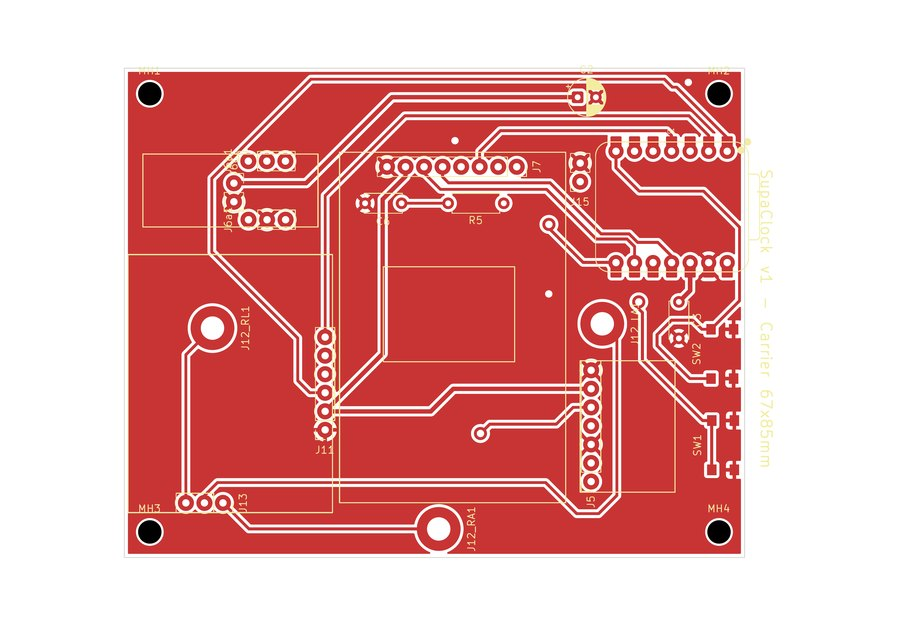
\includegraphics[width=\linewidth]{pcb_front_e4.jpg}
            \scriptsize Cara superior
        \end{minipage}
        \hfill
        \begin{minipage}{0.48\linewidth}
            \centering
            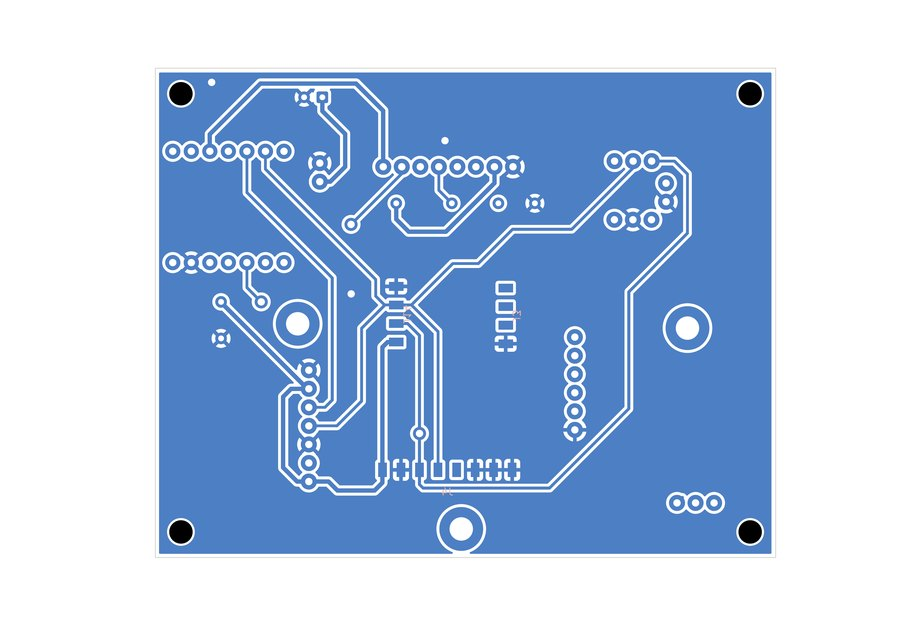
\includegraphics[width=\linewidth]{pcb_back_e4.jpg}
            \scriptsize Cara inferior
        \end{minipage}
        \column{0.46\textwidth}
        \footnotesize
        \textbf{Motivaci\'on del cambio}
        \begin{itemize}\itemsep0.12cm
            \item Reglas de fabricaci\'on m\'as finas que LPKF local.
            \item V\'ias y pistas m\'as peque\~nas para aumentar densidad.
            \item Mejor repetibilidad y acabado industrial.
            \item Reducci\'on de altura objetivo: \textbf{al menos 33\%}.
        \end{itemize}
        \vspace{0.15cm}
        \begin{block}{Meta geom\'etrica}
            \scriptsize Si el prototipo ronda 22\,mm de altura, una reducci\'on de 33\% apunta a una carcasa del orden de 15\,mm o menos. El valor final debe confirmarse con la placa ensamblada.
        \end{block}
    \end{columns}
\end{frame}

\begin{frame}{Redise\~no de carcasa final}
    \begin{columns}[T]
        \column{0.48\textwidth}
        \centering
        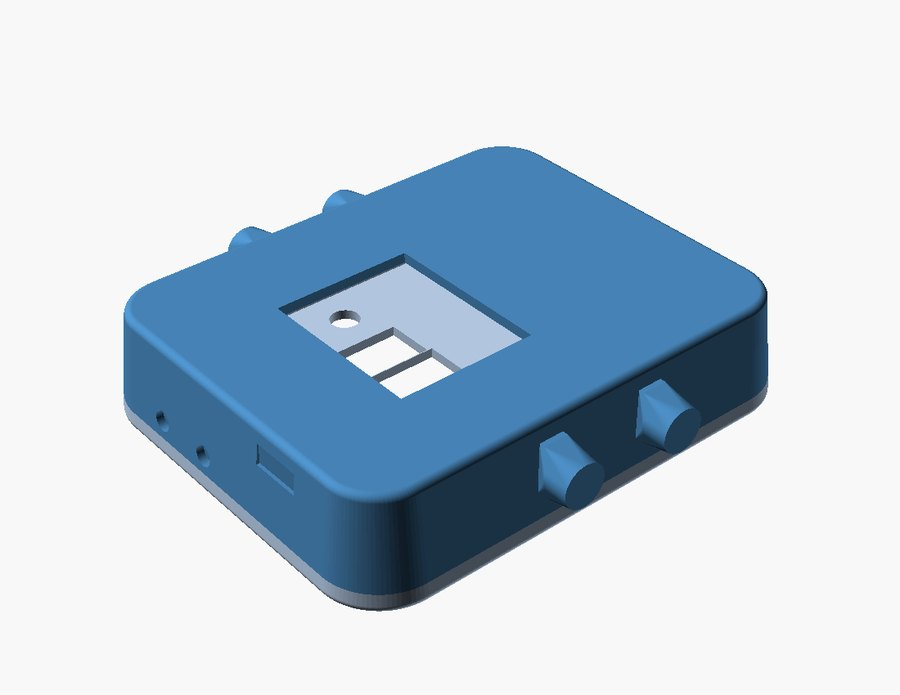
\includegraphics[width=0.95\linewidth]{case_hero_e4.jpg}
        \vspace{0.15cm}
        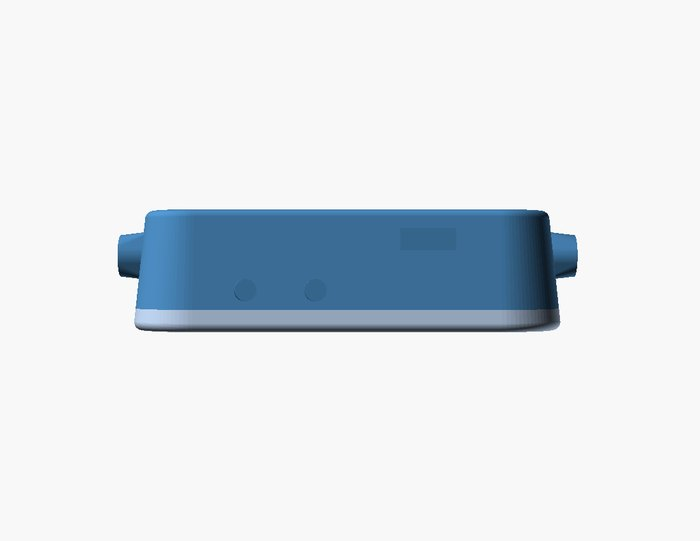
\includegraphics[width=0.48\linewidth]{case_side_e4.jpg}
        \column{0.52\textwidth}
        \footnotesize
        \textbf{Aprendizajes del prototipo funcional}
        \begin{itemize}\itemsep0.11cm
            \item La carcasa debe seguir a la PCB final, no al prototipo con headers.
            \item El contacto sensor-piel define calidad de PPG, temperatura y ECG.
            \item Botones, USB-C y electrodos requieren tolerancias reales.
            \item Debe poder abrirse/cerrarse sin cargar soldaduras ni pads.
            \item El dise\~no final debe priorizar altura, comodidad y acceso a sensores.
        \end{itemize}
        \begin{block}{Cambio conceptual}
            \scriptsize La carcasa ya no es una envolvente: participa directamente en la calidad de medici\'on biom\'etrica.
        \end{block}
    \end{columns}
\end{frame}

\section{Ruta al 100\%}

\begin{frame}{Qu\'e falta para completar el 100\%}
    \scriptsize
    \begin{columns}[T]
        \column{0.25\textwidth}
        \textbf{\textcolor{main}{Hardware}}
        \begin{itemize}\itemsep0.05cm
            \item Pedir PCB China.
            \item Bring-up el\'ectrico.
            \item Validar consumo.
            \item Ajustar electrodos ECG.
        \end{itemize}
        \column{0.25\textwidth}
        \textbf{\textcolor{main}{Software / ML}}
        \begin{itemize}\itemsep0.05cm
            \item Dataset final.
            \item Matriz de confusi\'on.
            \item Cuantizaci\'on final.
            \item UI de estado HAR.
        \end{itemize}
        \column{0.25\textwidth}
        \textbf{\textcolor{main}{Mec\'anica}}
        \begin{itemize}\itemsep0.05cm
            \item Carcasa compacta.
            \item Ventanas de sensores.
            \item Botones y USB-C.
            \item Confort y montaje.
        \end{itemize}
        \column{0.25\textwidth}
        \textbf{\textcolor{main}{Validaci\'on}}
        \begin{itemize}\itemsep0.05cm
            \item Demo cerrada.
            \item Pruebas repetibles.
            \item Informe final.
            \item Video/evidencia.
        \end{itemize}
    \end{columns}
    \vspace{0.32cm}
    \begin{alertblock}{Criterio de t\'ermino}
        \scriptsize El 100\% se logra cuando el reloj mide ECG/biometr\'ia, clasifica actividad y se puede usar cerrado con una placa/carcasa repetible.
    \end{alertblock}
\end{frame}

\begin{frame}{Plan de ataque: 90\% $\rightarrow$ 100\%}
    \centering
    \begin{tikzpicture}[
        node/.style={draw=main, rounded corners=5pt, fill=main!9, align=center, minimum width=2.65cm, minimum height=1.15cm, font=\scriptsize},
        done/.style={node, draw=accent, fill=accent!13},
        arr/.style={-Stealth, thick, main}
    ]
        \node[node] (a) {1. Fabricaci\'on\\Gerbers + pedido};
        \node[node, right=0.45cm of a] (b) {2. Bring-up\\rails + sensores};
        \node[done, right=0.45cm of b] (c) {3. Carcasa final\\altura + contacto};
        \node[done, right=0.45cm of c] (d) {4. Validaci\'on\\demo cerrada};
        \draw[arr] (a) -- (b);
        \draw[arr] (b) -- (c);
        \draw[arr] (c) -- (d);
    \end{tikzpicture}
    \vspace{0.45cm}
    \begin{block}{Riesgo principal}
        \footnotesize El tramo final no es un problema aislado de c\'odigo: combina tolerancias f\'isicas, ruido real, contacto con piel, energ\'ia y repetibilidad de ensamblaje.
    \end{block}
\end{frame}

\begin{frame}{Arquitectura integrada actualizada}
    \begin{columns}[T]
        \column{0.42\textwidth}
        \scriptsize
        \begin{tabular}{l l}
            \toprule
            \textbf{Bloque} & \textbf{Estado Entrega 4} \\
            \midrule
            BMI160 IMU & ML/CSV en uso \\
            MAX30102 PPG & integrado, validaci\'on final pendiente \\
            MAX30205 Temp. & integrado, offset carcasa pendiente \\
            MAX17048 Fuel & telemetr\'ia disponible \\
            AD8232 ECG & \textbf{funcionando en PCB} \\
            ST7789 Display & GUI funcional \\
            App m\'ovil & BLE + REC + dashboard \\
            TinyML HAR & Validaci\'on inercial (clean/noisy) \\
            PCB final & camino JLCPCB \\
            \bottomrule
        \end{tabular}
        \column{0.58\textwidth}
        \vspace{-0.25cm}
        \begin{flushright}
            \resizebox{1.02\linewidth}{!}{\begin{tikzpicture}[
    node distance=0.6cm and 0.9cm,
    every node/.style={font=\scriptsize},
    blockOK/.style={rectangle, rounded corners, draw=black!70, very thick, fill=green!22, text width=2.8cm, align=center, minimum height=0.95cm},
    blockPart/.style={rectangle, rounded corners, draw=black!70, very thick, fill=yellow!28, text width=2.8cm, align=center, minimum height=0.95cm},
    blockTodo/.style={rectangle, rounded corners, draw=black!70, very thick, dashed, fill=red!12, text width=2.8cm, align=center, minimum height=0.95cm},
    energy/.style={rectangle, rounded corners, draw=black!70, very thick, fill=orange!22, text width=2.6cm, align=center, minimum height=0.9cm},
    mcu/.style={rectangle, rounded corners, draw=black, very thick, fill=blue!22, text width=3.4cm, align=center, minimum height=1.4cm, font=\small\bfseries},
    busI2C/.style={->, >=stealth, thick, blue!70!black},
    busSPI/.style={->, >=stealth, thick, violet!80!black},
    adc/.style={->, >=stealth, thick, orange!85!black},
    gpio/.style={->, >=stealth, thick, teal!70!black},
    ble/.style={->, >=stealth, thick, dashed, blue!60},
    pwr/.style={->, >=stealth, thick, red!70},
    legend/.style={rectangle, draw=black!50, fill=white, inner sep=4pt}
]
% ============== MCU (Centro) ==============
\node[mcu] (mcu) {XIAO ESP32-S3\\FreeRTOS + LVGL 8.4\\\textbf{Funcionando}};

% ============== INTERFAZ LOCAL (Izquierda) ==============
\node[blockOK, left=2.2cm of mcu] (st7789) {ST7789 1.69" IPS\\\textbf{100\%} (LVGL)};
\node[blockOK, above=0.3cm of st7789] (btns) {2 botones GPIO\\\textbf{100\%} (debounce)};
\node[blockOK, below=0.3cm of st7789] (gui) {GUI: Home/Bio/Menu\\\textbf{100\%} (7 pant.)};

% ============== ENERGÍA (Arriba a la Izquierda) ==============
\node[energy, left=0.6cm of st7789] (sgm40567) {Cargador SGM40567\\\textbf{100\%} (XIAO S3)};
\node[energy, above=0.3cm of sgm40567] (sgm6029) {Buck SGM6029 3.3\,V\\\textbf{100\%} (XIAO S3)};
\node[blockOK, above=0.3cm of sgm6029] (fuel) {MAX17048\\\textbf{100\%} (I2C)};

\node[energy, left=0.6cm of sgm40567] (usbc) {USB-C\\\textbf{100\%} (XIAO S3)};
\node[energy, above=0.3cm of usbc] (bms) {BMS TP4056+DW01A\\\textbf{100\%} (Carrier)};
\node[energy, above=0.3cm of bms] (lipo) {Bater\'ia LiPo 3.7\,V\\\textbf{100\%} (502030)};

% ============== SENSORES I2C y ADC (Derecha) ==============
\node[blockOK, right=2.2cm of mcu, yshift=1.8cm] (max205) {MAX30205\\\textbf{100\%} \textit{(0x48)}};
\node[blockOK, below=0.3cm of max205] (bmi) {BMI160 IMU\\\textbf{100\%} \textit{(0x68)}};
\node[blockOK, below=0.3cm of bmi] (max102) {MAX30102\\\textbf{95\%} HR/SpO\textsubscript{2}};
\node[blockOK, below=0.3cm of max102] (ad8232) {AD8232 + DMA\\\textbf{100\%} \textit{(GPIO1)}};

% ============== ECOSISTEMA (Abajo) ==============
\node[blockOK, below=1.8cm of mcu] (ble) {BLE NimBLE\\\textbf{100\%} (3 GATT chr.)};
\node[blockOK, right=0.8cm of ble] (cli) {Cliente PC testing\\\textbf{100\%} (\texttt{logger})};
\node[blockOK, right=0.8cm of cli] (fb) {Firebase (Cloud Fn)\\\textbf{100\%} (Pan-Tomp.)};

\node[blockOK, below=0.6cm of ble] (app) {App m\'ovil (gateway)\\\textbf{90\%} (Flutter)};
\node[blockOK, right=0.8cm of app] (pcb) {PCB Carrier v1\\\textbf{100\%} (Listo)};
\node[blockPart, right=0.8cm of pcb] (ml) {TinyML (CNN 1D)\\\textbf{70\%} (Falta capt. datos)};

% ============== Conexiones de Potencia ==============
\draw[pwr] (usbc) -- (bms);
\draw[pwr] (lipo) -- (bms);
\draw[pwr] (lipo) -- (fuel);
\draw[pwr] (bms)  -- (sgm6029);
\draw[pwr] (usbc) -- (sgm40567);
\draw[pwr] (sgm40567) -- (sgm6029);
\draw[pwr] (sgm6029.west) -- ++(-0.2,0) |- ([yshift=0.4cm]fuel.north) -| ([xshift=-1.2cm]mcu.north);

% ============== Conexiones I2C ==============
\draw[busI2C] (fuel.east) -| ([xshift=-0.6cm]mcu.north);

% Enrutamiento ortogonal tipo "bus" para alinear sensores de la derecha
\draw[busI2C] (max205.west) -- ++(-0.6,0) |- node[right, pos=0.25, font=\tiny]{I2C 400\,kHz} ([yshift=0.5cm]mcu.east);
\draw[busI2C] (bmi.west)    -- ++(-0.6,0) |- ([yshift=0.15cm]mcu.east);
\draw[busI2C] (max102.west) -- ++(-0.6,0) |- ([yshift=-0.2cm]mcu.east);

% ============== Conexiones ADC ==============
\draw[adc] (ad8232.west) -- ++(-0.6,0) |- node[below, pos=0.75, font=\tiny]{ADC1 20\,kHz} ([yshift=-0.55cm]mcu.east);

% ============== Conexiones SPI/GPIO ==============
\draw[busSPI] (mcu.west) -- node[above]{SPI 80\,MHz} (st7789.east);
\draw[gpio] (btns.east) -- ++(0.4,0) |- node[above, pos=0.8, font=\tiny]{GPIO} ([yshift=0.4cm]mcu.west);

% ============== Conexiones Ecosistema ==============
\draw[ble] (mcu) -- (ble);
\draw[ble] (ble) -- node[above, font=\tiny, align=center]{GATT\\3 chr.} (cli);
\draw[gpio, ->] (cli) -- node[above]{Wi-Fi} (fb);
\draw[ble, ->] (ble) -- (app);
\draw[ble, ->] (app.south) -- ++(0,-0.4) -| (fb.south);

% ============== Leyenda ==============
\node[legend, below=1.2cm of pcb] (leg) {%
\begin{tabular}{ll}
\textcolor{green!50!black}{$\blacksquare$} Listo &
\textcolor{red!70}{\textbf{$\rightarrow$}} Potencia \\
\textcolor{yellow!60!black}{$\blacksquare$} Parcial &
\textcolor{blue!70!black}{$\rightarrow$} I2C 400\,kHz \\
\textcolor{red!70!black}{$\blacksquare$} Pendiente &
\textcolor{violet!80!black}{$\rightarrow$} SPI 80\,MHz \\
\textcolor{blue!60}{$\dashrightarrow$} BLE/Wi-Fi &
\textcolor{orange!85!black}{$\rightarrow$} ADC/DMA \\
\end{tabular}};
\end{tikzpicture}
}
            \vspace{0.05cm}\newline
            \scriptsize Arquitectura de hardware heredada de Entrega 3, ahora con ECG y app como evidencia central de integraci\'on.
        \end{flushright}
    \end{columns}
\end{frame}

\begin{frame}[plain]
    \centering
    \vspace{1.05cm}
    {\Huge \color{main} \textbf{Demostraci\'on / Discusi\'on}}\\[0.55cm]
    {\Large ECG en PCB + BLE + avances ML}\\[0.35cm]
    \footnotesize
    Placa final fabricada en China \textbar{} redise\~no de carcasa \textbar{} validaci\'on para cierre 100\%
    \vspace{0.75cm}
    \begin{block}{Mensaje final}
        \centering
        El proyecto ya demuestra funcionamiento; la etapa final convierte ese funcionamiento en un reloj repetible, compacto y defendible.
    \end{block}
\end{frame}

\end{document}
